\documentclass[10pt,letterpaper]{article}
\usepackage[margin=.85in]{geometry}
\usepackage[T1]{fontenc}\usepackage{lmodern,graphicx,booktabs,amsmath,xcolor,hyperref,xurl,caption,fancyhdr}
\hypersetup{colorlinks=true,urlcolor=teal,linkcolor=teal,pdftitle={Know where inspection labels are missing},pdfauthor={James Jean}}
\pagestyle{fancy}\fancyhf{}\fancyhead[L]{\small Inspection label coverage / Study 15}\fancyhead[R]{\small Independent descriptive audit}\fancyfoot[C]{\thepage}
\setlength{\headheight}{14pt}\setlength{\parindent}{0pt}\setlength{\parskip}{6pt}\captionsetup{font=small,labelfont=bf,hypcap=false}
\begin{document}
{\small\color{teal} ENVIRONMENTAL MONITORING / TRAINING-LABEL QUALITY\par}
\vspace{7pt}{\LARGE\bfseries Know where inspection labels are missing\par}
\vspace{6pt}James Jean \hfill 30 October 2026
\section*{The decision}
Before using inspection records to train a facility risk model, establish who has an observed outcome. In this captured cohort of \textbf{183,500 current operating air sources}, \textbf{13,613 (7.4\%)} have a recorded pass or fail stack-test result during 2021--2025. Another \textbf{169,698} have no dated stack-test record in the window. An absent national record cannot supply a passing outcome.

\textbf{Practical recommendation.} Use the complete state and source-class coverage summaries to direct data reconciliation. Confirm the required monitoring universe and comparable outcomes with the relevant source systems before building a risk queue. This project supplies the coverage audit and reproducible counts; improved detection, reduced effort and realized operational value have not been measured.

\begin{center}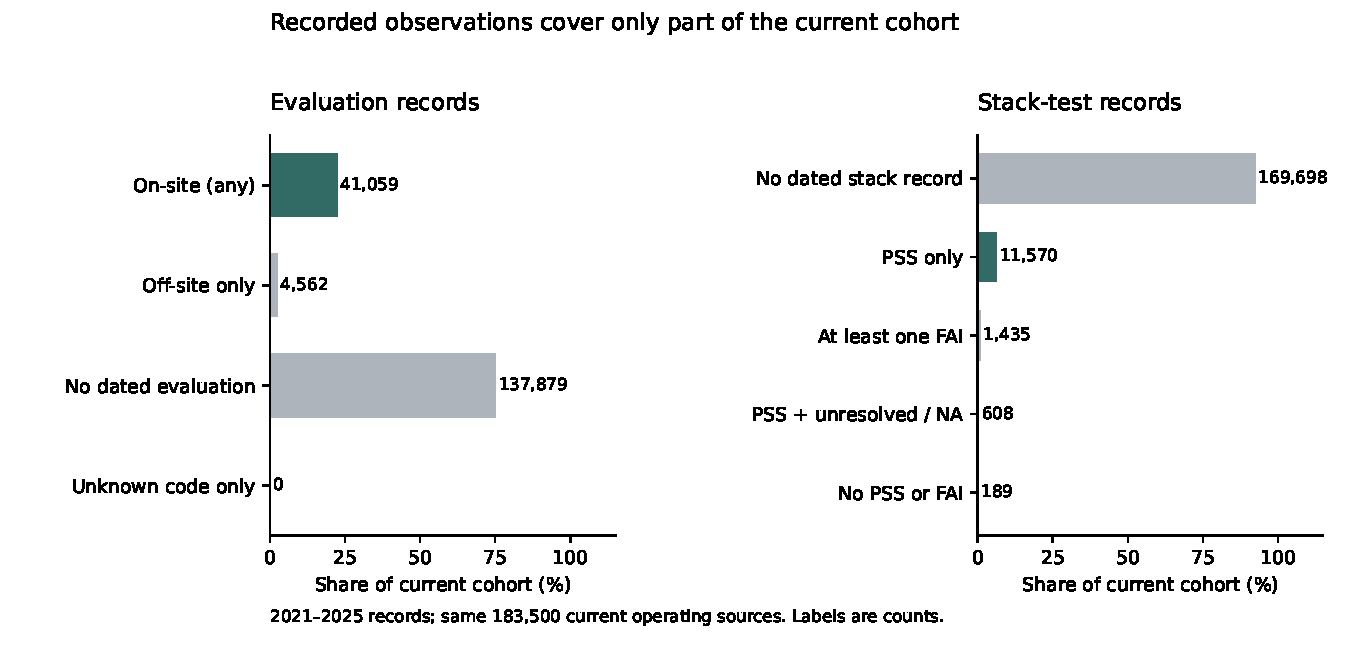
\includegraphics[width=\linewidth]{images/recorded_coverage.pdf}\end{center}
\captionof{figure}{Recorded evaluation and stack-test categories in the same current cohort. Bar lengths are percentages; printed labels are facility counts. PSS and FAI are source pass/fail codes, not a certification of current compliance. Unresolved includes pending, incomplete, not-applicable, blank or unrecognized tokens.}

\textbf{Important limits.} The data do not identify all facilities required to have a stack test. A missing record may reflect reporting rules, state-only records, source-system delay or no event. All windows use current operating status, so these are not historical national inspection rates. A historical failed test does not establish current noncompliance. No risk model, calibration, propensity correction or enforcement ranking is claimed.

\newpage
\section*{1. Source, current cohort and corrections}
EPA ECHO provides ICIS-Air bulk files for analyst and developer use [1]. This study captures one complete published ZIP on 30 October 2026, after the protocol commit. The archive is 69,872,864 bytes and reports last modification on 25 October 2026. Exact request times, HTTP status, member hashes and minimal projection hashes are retained in the source manifest.

\begin{center}\begin{tabular}{lr}\toprule
Captured table & Original rows\\\midrule
Current facility rows & 280,423 \\
Evaluation rows & 1,824,426 \\
Stack-test rows & 658,331 \\
\bottomrule\end{tabular}\end{center}

The cohort requires a nonempty program key, current operating status OPR, and a location in the fifty states or DC. All source facility identities are unambiguous under the selected attributes. The screen retains 183,500 facilities; 96,294 source rows are not OPR and 801 are outside the geographic scope. These reason counts overlap. Current class, operating status and surviving facilities do not reconstruct the population active in each historical year; entry dates and historical status remain unknown.

For each event table, exact duplicate selected records collapse. All records of conflicting (program, activity) identities are excluded. Evaluation records contain 149 conflicting identities covering 384 source rows, plus 398 duplicate excess rows among nonconflicting identities. Stack-test identities have no such conflicts or duplicate excess. All exclusions, orphan joins, dates outside the window and code tokens remain in the source audit; overlapping reasons must not be added as distinct events.

\textbf{Recorded correction.} The dictionary [2] describes slash-separated dates, but the evaluation export uses month-day-four-digit-year dates with dashes. The initial parser rejected every evaluation date. That output and code are retained privately as a failed run, not treated as absence of real evaluations. The corrected parser accepts this equivalent delimiter while preserving the cohort, windows and categories. The result is a corrected retrospective descriptive audit; no protected predictive test or post-hoc model selection is claimed. Four stack-test source dates remain invalid or missing and are reported separately.

Only factual codes, dates and full SHA256 source keys are public in 29 fixed-size shards. Original archives and identity mappings stay private. No names, addresses, contacts or coordinates are in the projections. Hashes minimize direct exposure but do not guarantee anonymity. EPA provides no warranty of complete or current reporting [3]; there is no blanket CC0 or ownership claim over submitted state/local content. Separate formal-publication projects remain private.

\newpage
\section*{2. Source classes have different observation coverage}
Current reported source class is retained without assuming it measures actual emissions, risk or required monitoring. The denominator below is the same current cohort, partitioned by current class. Missing class remains visible.

\begin{center}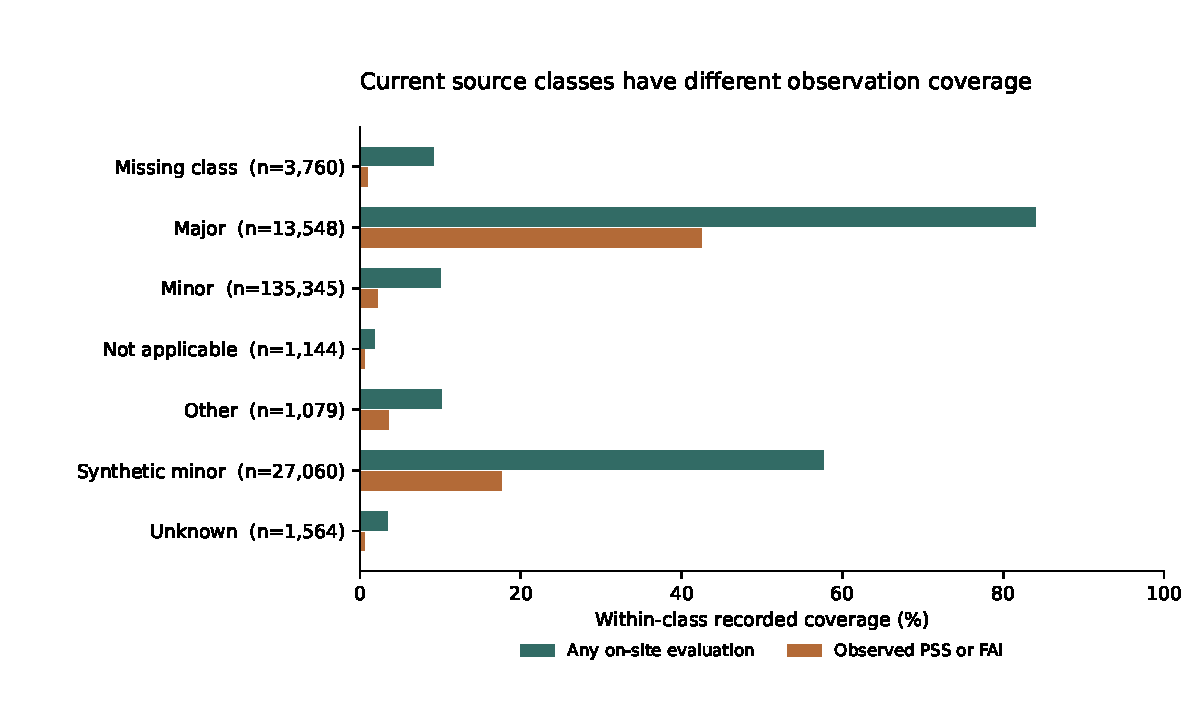
\includegraphics[width=.97\linewidth]{images/class_coverage.pdf}\end{center}
\captionof{figure}{Combined 2021--2025 recorded coverage by current source class. Any on-site evaluation and an observed PSS/FAI stack-test result are separate indicators; they need not refer to the same event. Every observed class is retained.}

\begin{center}\small\begin{tabular}{lrrrr}\toprule
Current class & Facilities & Full on-site & Any on-site & Stack PSS/FAI\\\midrule
Missing class & 3,760 & 276 & 343 & 34 \\
Major & 13,548 & 11,311 & 11,382 & 5,754 \\
Minor & 135,345 & 9,648 & 13,544 & 2,995 \\
Not applicable & 1,144 & 9 & 20 & 6 \\
Other & 1,079 & 94 & 109 & 38 \\
Synthetic minor & 27,060 & 15,008 & 15,607 & 4,777 \\
Unknown & 1,564 & 30 & 54 & 9 \\
\bottomrule\end{tabular}\end{center}

Major and minor classes differ substantially in observed coverage. That contrast is not evidence that one class is safer, that an agency performs better, or that required tests were missed. EPA describes different reporting completeness and monitoring practices across facility types, including state-only information for some smaller facilities [3]. Those mechanisms are not identified from these counts. Training and evaluation restricted to the observed subset require a separate justification before extending conclusions to the unobserved population.

\newpage
\section*{3. All annual comparisons remain visible}
Use each calendar year 2021--2025 and the combined window, without choosing a favorable year. Full on-site evaluation is a subset of any on-site evaluation. Off-site-only sources have an off-site record but no on-site record within the same window; an off-site review is not counted as a visit.

\begin{center}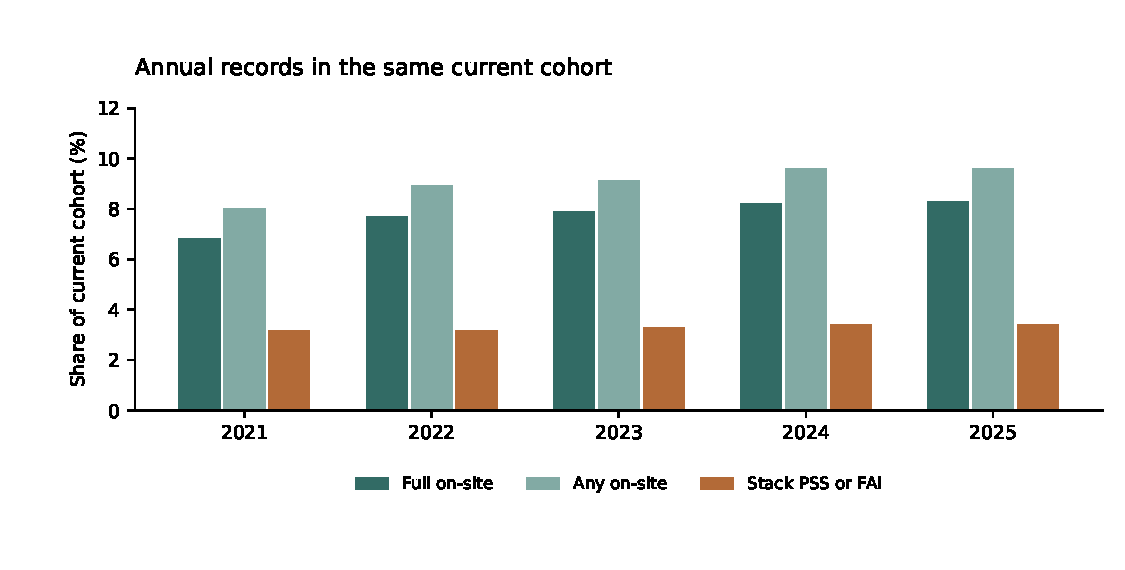
\includegraphics[width=.98\linewidth]{images/annual_coverage.pdf}\end{center}
\captionof{figure}{Each year uses the same 183,500 current operating sources. Differences across annual bars do not establish changes in historical inspection rates, agency performance or required monitoring: current-cohort selection, source entry and reporting revisions remain unresolved.}

\begin{center}\small\begin{tabular}{lrrrrrr}\toprule
Year & Full on & Any on & Off only & No eval. & Unknown only & Stack PSS/FAI\\\midrule
2021 & 12,510 & 14,712 & 6,772 & 162,013 & 3 & 5,806 \\
2022 & 14,156 & 16,363 & 5,211 & 161,924 & 2 & 5,830 \\
2023 & 14,485 & 16,776 & 4,543 & 162,177 & 4 & 6,013 \\
2024 & 15,053 & 17,602 & 3,715 & 162,180 & 3 & 6,258 \\
2025 & 15,258 & 17,600 & 3,777 & 162,120 & 3 & 6,228 \\
\bottomrule\end{tabular}\end{center}

In the combined window, 41,059 sources have an on-site evaluation, 4,562 have only off-site evaluations and 137,879 have no dated evaluation in this source/window. These three counts plus the unknown-code-only category partition the cohort. Unknown monitoring codes are retained rather than assigned to on-site or off-site after seeing the results. The complete code audit preserves these exceptions.

The same source can have many evaluations or tests. Facility coverage counts each source once per indicator and window. Event totals are a different denominator: after identity and date rules, 221,912 evaluation events and 157,168 stack-test events join the current cohort in the combined window. Neither event count is a count of unique facilities or a number of enforcement findings.

\newpage
\section*{4. Missing records do not define passing outcomes}
The stack-test partition retains every current source. At least one FAI takes precedence over other statuses; the group can contain both pass and fail records. PSS only requires at least one PSS and no FAI, pending, incomplete, not-applicable, blank or unknown result token in the window. Other categories preserve unresolved or noncomparable observations.

\begin{center}\small\begin{tabular}{lrr}\toprule
Combined-window recorded category & Sources & Share\\\midrule
No dated stack-test record & 169,698 & 92.5\% \\
At least one FAI & 1,435 & 0.8\% \\
PSS only & 11,570 & 6.3\% \\
PSS plus unresolved / NA / unknown & 608 & 0.3\% \\
Records but no PSS or FAI & 189 & 0.1\% \\
\bottomrule\end{tabular}\end{center}

Among sources with at least one FAI, 1,213 also have PSS records. The audit does not infer the order, regulatory resolution, equivalent test conditions or current legal status from the presence of both tokens. A PSS result also does not establish compliance with every applicable requirement. A stack test and a full or partial facility evaluation are different observations [2].

The complete data-review list includes every state and class group, ordered by the count with no dated stack-test record and a fixed group/name tie break. It is a list for source reconciliation, not a facility inspection or enforcement priority. State and class groups overlap; their counts must not be summed. A high count or rate of absent records does not establish that a test was required or that missingness is random.

\textbf{What a risk-model study still needs.} Define a decision and comparable outcome, establish the eligible required-monitoring universe, reconcile state/local and national records, and document feature availability before each decision. Evaluate how observations were selected; this audit supplies no defensible observation propensity or missing-at-random assumption. Separate future evaluation data and independent outcome review would be needed to compare a predictive queue. No classification accuracy, AUC, probability calibration or counterfactual inspection gain follows from coverage counts.

These are exact descriptive counts of a captured cohort, not a random sample used to estimate national prevalence. Sampling intervals and significance tests would obscure the unresolved coverage and measurement problems. The practical recommendation is to establish labels and their observation process before fitting a risk model. No scientific novelty can be inferred from running an audit.

\newpage
\section*{5. Reproducibility, scope and next evidence}
Independent Pandas parsing reconciles the minimal projections against the private ZIP: 39,720,857 assertions pass. Separate SQLite code rebuilds raw identity conflicts, current-cohort eligibility, date joins and indicators without importing analysis helpers. It verifies all 1,101,000 facility-window rows, 17,616,000 observation fields and 354 group rows through two-way set equality and exact count checks. Seventeen finite hand-authored fixtures cover dates, duplicates, identity conflicts, no records, off-site reviews and mixed results. Synthetic fixtures are excluded from the research counts.

An offline replay regenerates the observation and group exports in an owned temporary directory, matches 17,622,640 CSV fields and one JSON document, reruns the fixtures and verifies published originals remain unchanged. It makes no network requests. Public source checks establish recorded hashes and schema; only the private-original mode performs the full source reconciliation. Three original figures are linked to source values and rendered geometry. Manuscript values are independently rebuilt from the observation exports. These finite checks do not prove universal correctness or complete reporting.

The date-delimiter failure and the original unsharded projection are preserved privately. Splitting the same selected records into 29 gzip shards solves file-size packaging without changing values or scope. The protocol, corrected retrospective qualification, exclusions and source uncertainty remain inspectable. No learned model, tuning grid, propensity weighting or protected predictive test was executed, so none is presented as a project skill or result.

Selective-label evaluation is established research, including Lakkaraju et al. [4]. Environmental inspection allocation using machine learning is also established, including Hino, Benami and Brooks [5], whose water-program target and evaluation are different from this air-source coverage audit. This project does not reproduce their models or inherit their benefit estimates. It contributes a transparent, current-snapshot diagnostic and reproducible data checks, not a new estimator or an exhaustive novelty claim.

\textbf{Next useful evidence.} Reconcile the low-coverage groups with state/local records, establish required monitoring and comparable outcomes, then design an evaluation that addresses selection. Record actual review effort and findings before claiming useful detection, saved time or other realized benefit. No deployment, accessibility conformance, operational adoption or legal-compliance assessment has been verified.

\small\textbf{Sources and prior work}\par
{\raggedright
{[1]} EPA ECHO, Data Downloads. \url{https://echo.epa.gov/tools/data-downloads}\par
{[2]} EPA ECHO, ICIS-Air dictionary. \url{https://echo.epa.gov/tools/data-downloads/icis-air-download-summary}\par
{[3]} EPA ECHO, About the Data. \url{https://echo.epa.gov/resources/echo-data/about-the-data}\par
{[4]} Lakkaraju et al. (2017), The Selective Labels Problem. \url{https://doi.org/10.1145/3097983.3098066}\par
{[5]} Hino, Benami and Brooks (2018), Machine learning for environmental monitoring. \url{https://doi.org/10.1038/s41893-018-0142-9}\par}
\end{document}
